\documentclass{article}
\usepackage[utf8]{inputenc}
\usepackage[T1]{fontenc}
\usepackage[english]{babel}
\setlength{\parindent}{0pt}
\usepackage{hyperref}
\hypersetup{
    colorlinks=true,
    linkcolor=blue,
    filecolor=magenta,      
    urlcolor=cyan}
\usepackage{graphicx}
\graphicspath{ {./pic/} }
\usepackage{multicol}
\usepackage{lscape}

\usepackage{fourier,amssymb,microtype,amsmath,gensymb}
\newcommand{\R}{\mathbb{R}}
\usepackage{mdframed,caption,xcolor}
\usepackage{tikz,tkz-euclide}

\title{Seminar 12. Auctions and previous exam problems}
\author{Xiaoguang Ling \\  \href{xiaoguang.ling@econ.uio.no}{xiaoguang.ling@econ.uio.no}}
\date{\today}

\begin{document}

\maketitle

%%%%%%%%%%%%%%%%%%%%%%%%%%%%%%%%%%%%%%%%%%%%%%%%%%%%%%%%%%%%%%%%%%%%%%%%%%%%%%%%%%%%%%%%%%%%%%
\section{Jehle \& Reny pp.484, exercise 9.2}

Show in two ways that the symmetric equilibrium bidding strategy of a first-price auction with $N$
symmetric bidders each with values distributed according to $F$, can be written as


$$\hat{b}(v) = v -\int_{0}^{v} \left(\frac{F(x)}{F(v)}\right)^{N-1} dx$$

For the first way, use our solution from the text and apply integration by parts. For the second
way, use the fact that $F^{N-1}(r)(v - \hat{b}(r))$ is maximised in r when $r = v$ and then apply the envelope
theorem to conclude that $d(F^{N-1}(v)(v - \hat{b}(v))/dv = F^{N-1}(v)$; now integrate both sides from $0$ to $v$.

\bigskip

See lecture notes for the third lecture on the economics of information (on ``Auctions and the revenue equivalence theorem''), pages 17 and 19.


\section{Jehle \& Reny pp.484, exercise 9.1 - Show that the bidding strategy in (9.5) is strictly increasing.}

By exercise 9.1, the bid function can be written as:$$\hat{b}(v_i) = v_i - \frac{\int_0^{v_i}[F(x)]^{N-1} dx}{[F(v_i)]^{N-1}} \, .$$

Then:

\begin{align*}
  \frac{d}{dv_i}\left( \hat{b}(v_i) \right) &= \frac{d}{dv_i}\left( v_i - \frac{\int_0^{v_i}[F(x)]^{N-1} dx}{[F(v_i)]^{N-1}} \right) \\
  &= 1 - \frac{[F(v_i)]^{N-1}}{[F(v_i)]^{N-1}} + \frac{\int_0^{v_i}[F(x)]^{N-1} dx }{[F(v_i)]^{2N-2}} \cdot \frac{d}{dv_i}\left( [F(v_i)]^{N-1} \right) \\
  &= \frac{\int_0^{v_i}[F(x)]^{N-1} dx }{[F(v_i)]^{2N-2}} \cdot (N-1) [F(v_i)]^{N-2} f(v_i) > 0 \, .
\end{align*}

\bigskip

\section{Jehle \& Reny pp.485, exercise 9.3}

This exercise will guide you through the proof that the bidding function in (9.5) is in fact a symmetric
equilibrium of the first-price auction.

\subsection*{(a)} Recall from (9.2) that
$$\frac{du(r,v)}{dr}=(N-1)F^{N-2}(r)f(r)(v-\hat{b}(r))-F^{N-1}(r)\hat{b'}(r).$$
Using (9.3), show that


\begin{align*}
\frac{du(r,v)}{dr}&=(N-1)F^{N-2}(r)f(r)(v-\hat{b}(r))-(N-1)F^{N-2}(r)f(r)(r-\hat{b'}(r)) \\
&= (N-1)F^{N-2}(r)f(r)(v-r)
\end{align*}

\subsection*{(b)}Use the result in part (a) to conclude that $du(r, v)/dr$ is positive when $r < v$ and negative when
$r > v$, so that $u(r, v)$ is maximised when $r = v$.

\section{Problems 2  of the exam in \href{https://www.uio.no/studier/emner/sv/oekonomi/ECON4240/previous-exams/}{ECON4240, Spring 2005}}

Consider a strategic situation between an employer ($E$) and a worker ($W$). $E$ can either accept
($A$) or reject ($R$) $W$. $W$ can either become skilled ($S$) through education, or remain unskilled
($U$). $W$ can be of two types; either he is inherently high ability ($H$) or he is inherently low
ability ($L$). The players' payoffs depending on their actions and W's type is shown below.

{\centering
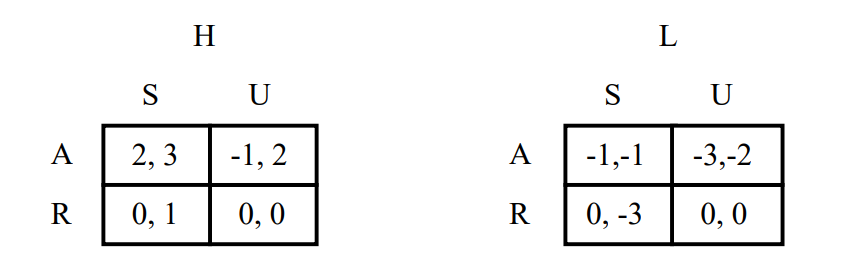
\includegraphics[width=0.8\textwidth]{12.q2}
\vspace{2mm}}


\subsection*{a) Rationalizable strategies \& NE} For each of these games, determine the set of (pure) rationalizable strategies for each
player, and the set of pure-strategy Nash equilibria.

\bigskip

In Game $H$: Only $S$ and $A$ are rationalizable. $(S, A)$ is the unique NE. 

In Game $L$. Only $U$ and $R$ are rationalizable. $(U, R)$ is the unique NE.


\subsection*{b) Bayesian normal form} Assume next that only $W$ knows his own type, while player $E$ thinks that the two types
of $W$ are equally likely. Model this situation in an ex ante perspective by specifying
the Bayesian normal form.

\bigskip

Denote the Worker's contingent choices are: If Game $H$, $S$ and $U$; If Game $L$, $S'$ and $U'$. The Baysian normal form is:


\begin{center}
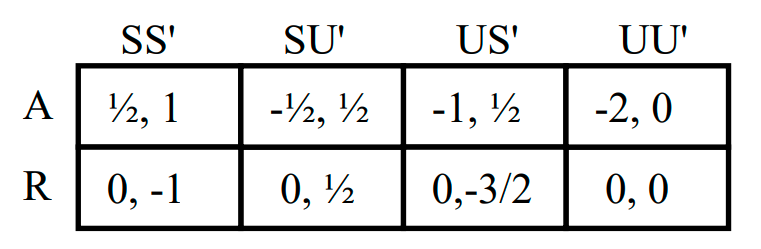
\includegraphics[width=0.6\textwidth]{12.q2_2}
\vspace{2mm}
\end{center}


\subsection*{c) Rationalizable strategy \& BNE} For the Bayesian normal form found in part (b), determine the set of (pure)
rationalizable strategies for each player, and the set of pure-strategy and/or mixedstrategy Nash equilibria.

\bigskip

\begin{center}
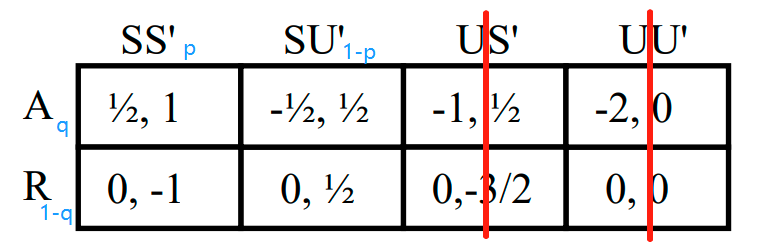
\includegraphics[width=0.6\textwidth]{12.q2_3}
\vspace{2mm}
\end{center}


\textbf{(1) Rationalizable strategy}

\medskip

For the Worker, $US'$ is dominated by $SS'$; $UU'$ is dominated by $SU'$. The rationalizable strategies are $SS$ and $SU'$.

\medskip

For the Employer, both $A$ and $R$ are rationalizable.

\medskip

\textbf{(2) Pure-strategy NE}

$$(A,SS'),(R,SU')$$

\smallskip

\textbf{(3) Mixed-strategy NE}

\medskip

Since $US'$ and $UU'$ are dominated, the Employer believes the Worker will choose 
them with probability (0,0).

\medskip

The Employer believes the Worker chooses $SS'$ and $SU'$ with probability $(p,1-p)$;
The Worker believe the Employer chooses $A$ and $R$ with probability $(q,1-q)$.

$$E(U^E_A) = p \times 0.5 + (1-p) \times (-0.5) = p-0.5$$
$$E(U^E_R) = p \times 0 + (1-p) \times 0 = 0$$
$$E(U^E_A) = E(U^E_R) \Rightarrow p=0.5$$


$$E(U^W_{SS'}) = q \times 1 + (1-q) \times (-1) = 2q-1$$
$$E(U^W_{SU'}) = q \times 0.5 + (1-q) \times 0.5 = 0.5$$
$$E(U^W_{SS'}) = E(U^W_{SU'}) \Rightarrow 2q-1=0.5 \Rightarrow \tfrac34$$

The Mixed-strategy NE is: the Employer chooses $A$ and $R$ with probability $(0.5,0.5)$; Worker chooses $SS'$ and $SU'$ with probability $(\tfrac34,\tfrac14)$.

\section{Problems 3  of the exam in \href{https://www.uio.no/studier/emner/sv/oekonomi/ECON4240/previous-exams/}{ECON4240, Spring 2005}}

Problem 3 (20 \%)
Consider again the strategic situation between an employer ($E$) and a worker ($W$) described in
Problem 2. Assume (as in parts b and c) of Problem 2) that only $W$ knows his own type, while
player $E$ thinks that the two types of $W$ are equally likely.
\subsection*{a) (Screening)} Assume now that $E$ acts before W, and that $E$'s choice of A or R can be
observed by $W$ before he makes his choice of $S$ or $U$. Show that there is a unique
subgame perfect Nash equilibrium.

\medskip

\textbf{Extensive Form:}

\begin{center}
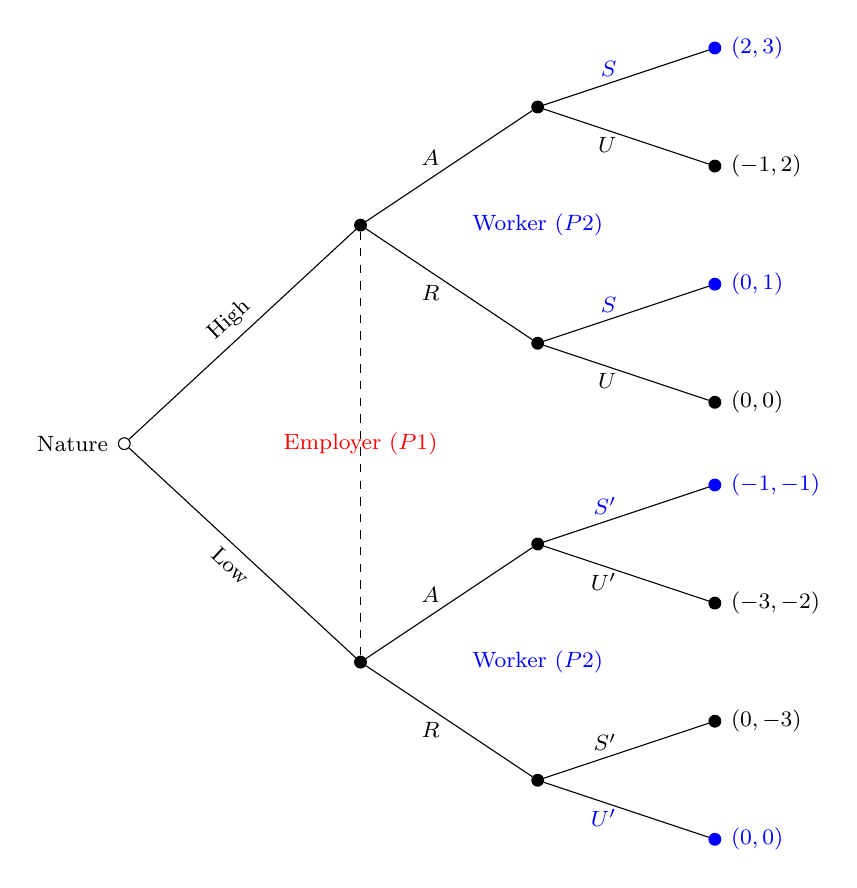
\begin{tikzpicture}[scale=1.5,font=\footnotesize]
\tikzset{
% Two node styles for game trees: solid and hollow
solid node/.style={circle,draw,inner sep=1.5,fill=black},
hollow node/.style={circle,draw,inner sep=1.5}
}
% Specify spacing for each level of the tree
\tikzstyle{level 1}=[level distance=20mm,sibling distance=37mm]
\tikzstyle{level 2}=[level distance=15mm,sibling distance=20mm]
\tikzstyle{level 3}=[level distance=15mm,sibling distance=10mm]
\tikzstyle arrowstyle=[scale=1]
\tikzstyle directed=[postaction={decorate,decoration={markings,
mark=at position .5 with {\arrow[arrowstyle]{stealth}}}}]

% The Tree
\node(0)[hollow node,label=left:{Nature}]{}[grow=east]
child{node(1)[solid node]{}
child{node(3)[solid node]{}
child{node[solid node,blue,label=right:{\textcolor{blue}{$(0,0)$}}]{}edge from parent node[left,blue,yshift=-3]{$U'$}}
child{node[solid node,label=right:{$(0,-3)$}]{}edge from parent node[left,yshift=3]{$S'$}}
edge from parent node[left,yshift=-3]{$R$}}
child{node(4)[solid node]{}
child{node[solid node,label=right:{$(-3,-2)$}]{}edge from parent node[left,yshift=-3]{$U'$}}
child{node[solid node,blue,label=right:{\textcolor{blue}{$(-1,-1)$}}]{}edge from parent node[left,blue,yshift=3]{$S'$}}
edge from parent node[left,yshift=3]{$A$}
}
edge from parent node [midway, below, sloped] (TextNode) {Low}
}
child{node(2)[solid node]{}
child{node(5)[solid node]{}
child{node[solid node,label=right:{$(0,0)$}]{}edge from parent node[left,yshift=-3]{$U$}}
child{node[solid node,blue,label=right:{\textcolor{blue}{$(0,1)$}}]{}edge from parent node[left,blue,yshift=3]{$S$}}
edge from parent node[left,yshift=-3]{$R$}}
child{node(6)[solid node]{}
child{node[solid node,label=right:{$(-1,2)$}]{}edge from parent node[left,yshift=-3]{$U$}}
child{node[solid node,blue,label=right:{\textcolor{blue}{$(2,3)$}}]{}edge from parent node[left,blue,yshift=3]{$S$}}
edge from parent node[left,yshift=3]{$A$}
}
edge from parent node [midway, above, sloped] (TextNode) {High}
};
% information set
\draw [dashed] (2) -- (1) ;
% specify mover
\node at ($(1)!.5!(2)$) {\textcolor{red}{Employer ($P1$)}};
\node at ($(5)!.5!(6)$) {\textcolor{blue}{Worker ($P2$)}};
\node at ($(3)!.5!(4)$) {\textcolor{blue}{Worker ($P2$)}};
\end{tikzpicture}
\end{center}

\medskip

The strategy of the $Worker$:
\begin{itemize}
\item If High:
\begin{itemize}
\item when $E$ chooses $A$, $W$ chooses $S$
\item when $E$ chooses $R$, $W$ chooses $S$
\end{itemize}
\item If Low:
\begin{itemize}
\item when $E$ chooses $A$, $W$ chooses $S'$
\item when $E$ chooses $R$, $W$ chooses $U'$
\end{itemize}
\end{itemize}

For the $Employer$:

$$E(U^E_A) = \tfrac12 \times 2 +\tfrac12 \times (-1) = 0.5$$
$$E(U^E_R) = \tfrac12 \times 0 +\tfrac12 \times 0 = 0$$
$$\Rightarrow E(U^E_A) > E(U^E_R)$$

The strategy of the $Employer$ is to choose $A$.

\medskip

Therefore there is a SPNE:

\{(For High ability Worker:) $S$ after $A$, $S$ after $R$. (For Low ability Worker:) $S'$ after $A$, $U'$ after $R$ ; (For Employer) $A$\}

\subsection*{b) (Signaling)} Assume now that $W$ acts before $E$, and that $W$'s choice of $S$ or $U$ can be
observed by $E$ before she makes her choice of $A$ or $R$. Show that there is a unique
perfect Bayesian equilibrium.

\medskip

\textbf{Extensive Form:}

\medskip

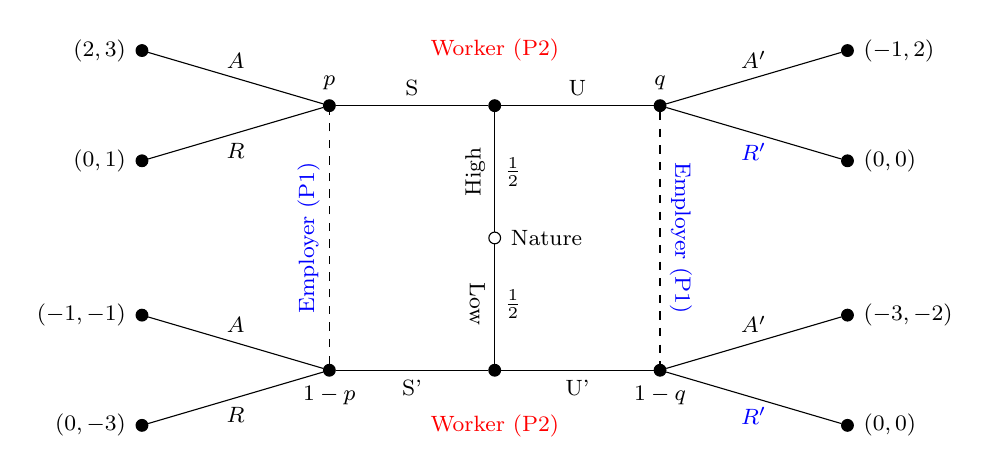
\begin{tikzpicture}[scale=1.4,font=\footnotesize]
\tikzset{
% Two node styles for game trees: solid and solid
solid node/.style={circle,draw,inner sep=1.5,fill=black},
hollow node/.style={circle,draw,inner sep=1.5}}
% Specify spacing for each level of the tree
\tikzstyle{level 1}=[level distance=12mm,sibling distance=25mm]
\tikzstyle{level 2}=[level distance=15mm,sibling distance=15mm]
\tikzstyle{level 3}=[level distance=17mm,sibling distance=10mm]
% The Tree
\node(0)[hollow node,label=right:{Nature}]{}
child[grow=up]{node[solid node,label=above:{
\begin{tabular}{c}
\textcolor{red}{Worker (P2)} \\ \\
\end{tabular}}] {}
child[grow=left]{node(1)[solid node,label=above:{$p$}]{}
child{node[solid node,label=left:{$(2,3)$}]{} edge from parent node [above]{$A$}}
child{node[solid node,label=left:{$(0,1)$}]{} edge from parent node [below]{$R$}}
edge from parent node [above]{S}}
child[grow=right]{node(3)[solid node,label=above:{$q$}]{}
child{node[solid node,label=right:{$(0,0)$}]{} edge from parent node [below]{\textcolor{blue}{$R'$}}}
child{node[solid node,label=right:{$(-1,2)$}]{} edge from parent node [above]{$A'$}}
edge from parent node [above]{U}
}
edge from parent node [right]{$\tfrac12$} node [midway, above, sloped] (TextNode){High}
}
child[grow=down]{node[solid node,label=below:{\begin{tabular}{c}
\\ \textcolor{red}{Worker (P2)}
\end{tabular}}] {}
child[grow=left]{node(2)[solid node,label=below:{$1-p$}]{}
child{node[solid node,label=left:{$(-1,-1)$}]{} edge from parent node [above]{$A$}}
child{node[solid node,label=left:{$(0,-3)$}]{} edge from parent node [below]{$R$}}
edge from parent node [below]{S'}
}
child[grow=right]{node(4)[solid node,label=below:{$1-q$}]{}
child{node[solid node,label=right:{$(0,0)$}]{} edge from parent node [below]{\textcolor{blue}{$R'$}}}
child{node[solid node,label=right:{$(-3,-2)$}]{} edge from parent node [above]{$A'$}}
edge from parent node [below]{U'}
}
edge from parent node [right]{$\tfrac12$} node[midway, below, sloped] (TextNode){Low}
};
% information set
\draw [dashed] (2) -- (1) node [midway, above, sloped, blue] (TextNode) {Employer (P1)};
\draw [dashed] (3) -- (4) node [midway, above, sloped, blue] (TextNode) {Employer (P1)};
\end{tikzpicture}


\medskip

The Worker has 4 possible strategies: $SS',UU',SU',US'$. 

\smallskip

Denote the updated belief of the Worker :
\begin{itemize}
\item $Pr(\text{Strong} | P/P') = p$
\item $Pr(\text{Weak} | U/U') = q$
\end{itemize}


\textbf{(1) When the Employer believes the Worker chooses $SS'$}

Then $p=Pr(\text{High})=0.5$,

$$E[U^E_{A}] = 0.5 \times 2+ 0.5\times (-1) = 0.5$$
$$E[U^E_{R}] = 0.5 \times 0+ 0.5 \times 0 = 0$$
$$E[U^E_{A}]>E[U^E_{R}]$$

The BR of the Employer is to choose $A$.

\smallskip

If the Worker surprisingly chooses $U/U'$, we can see that $R'$ dominates $A'$
for the Employer. Therefore, the Low ablility Worker will deviate from $S'$ to $U'$
to have a higher payoff ($U'$ and $R'$ leads to $(0,0)$)

\smallskip

$\Rightarrow SS'$ is not part of a PBE.

\medskip

\textbf{(2) When the Employer believes the Worker chooses $UU'$}

\smallskip

Since $R'$ dominates $A'$, the Employer will always choose $R'$. 
For a High ability Worker, deviating from $U$ to $S$ will always lead to
higher payoff (either 3 or 1), no matter how the Employer reacts.

\smallskip

$\Rightarrow UU'$ is not part of a PBE.

\medskip

\textbf{(3) When the Employer believes the Worker chooses $SU'$}

\smallskip

Then $p=1,q=0$,

\smallskip

The BR of the Employer is to choose $A$ after $S/S'$ (payoff is be $(2,3)$) and $R'$ after $U/U'$(payoff is be $(0,0)$).

\smallskip

If the High ability Worker eviates to $U$, the payoff is $(0,0)$, lower than $(2,3)$;
If the Low ability Worker eviates to $S$, the payoff is $(-1,-1)$, lower than $(0,0)$;

\smallskip

There is no incentive for the Worker to deviate.
$\Rightarrow SU'$ is part of a PBE.

\medskip

\textbf{(4) When the Employer believes the Worker chooses $US'$}

\smallskip

Then $p=0,q=1$,

\smallskip

The BR of the Employer is to choose $A$ after $S/S'$ and $R$ after $U/U'$.

\smallskip

For a Low ability Worker, deviating from $S'$ to $U'$ will increase the payoff from
$(-1,-1)$ to $(0,0)$.

\smallskip

$\Rightarrow US'$ is not part of a PBE.

\medskip

In conclusion, there is only one PBE:
$$\{SU',AR',p=1,q=0\}$$










\end{document}
